\section{RFC-0009: Session Start
Protocol}\label{rfc-0009-session-start-protocol}

\begin{itemize}
\tightlist
\item
  \textbf{RFC Number:} 0009
\item
  \textbf{Title:} Session Start Protocol
\item
  \textbf{Status:} Implementation
\item
  \textbf{Author(s):} Tino Breddin (@tolbrino), Lukas Pohanka
  (@NumberFour8)
\item
  \textbf{Created:} 2025-08-20
\item
  \textbf{Updated:} 2025-09-05
\item
  \textbf{Version:} v0.1.0 (Draft)
\item
  \textbf{Supersedes:} N/A
\item
  \textbf{Related Links:}
  \href{../RFC-0002-mixnet-keywords/0002-mixnet-keywords.md}{RFC-0002},
  \href{../RFC-0004-hopr-packet-protocol/0004-hopr-packet-protocol.md}{RFC-0004},
  \href{../RFC-0008-session-protocol/0008-session-protocol.md}{RFC-0008},
  \href{../RFC-0011-application-protocol/0011-application-protocol.md}{RFC-0011}
\end{itemize}

\subsection{1. Abstract}\label{1-abstract}

This RFC specifies the HOPR Session Start Protocol, a handshake protocol
for establishing sessions between peers in the HOPR mixnet. The protocol
manages session establishment, lifecycle, and capability negotiation
using HOPR packets as transport. It provides a standardized method for
initiating communication sessions, exchanging session parameters, and
maintaining session state through keep-alive mechanisms.

\subsection{2. Motivation}\label{2-motivation}

The HOPR mixnet requires a standardized mechanism for establishing
communication sessions between nodes. While the Session Data Protocol
(see
\href{../RFC-0008-session-protocol/0008-session-protocol.md}{RFC-0008})
handles data transmission, there needs to be a separate protocol for:

\begin{itemize}
\tightlist
\item
  Establishing sessions with capability negotiation
\item
  Exchanging session identifiers and targets
\item
  Managing session lifecycle and state
\item
  Providing error handling for session establishment failures
\item
  Maintaining session liveness through keep-alive mechanisms
\end{itemize}

The Session Start Protocol fills this gap by providing a lightweight,
transport-agnostic handshake mechanism specifically designed for the
HOPR ecosystem.

\subsection{3. Terminology}\label{3-terminology}

\begin{itemize}
\item
  \textbf{Challenge}: A 64-bit random value used to correlate requests
  and responses in the handshake process. Challenge values are
  interpreted as big-endian unsigned integers.
\item
  \textbf{Session Target}: The destination or purpose of a session,
  typically an address or service identifier, encoded in CBOR format.
\item
  \textbf{Session Capabilities}: A bitmap of session features and
  options negotiated during session establishment.
\item
  \textbf{Session ID}: A unique identifier assigned by the responder to
  identify the established session.
\item
  \textbf{Entry Node}: The node that initiates a session establishment
  request.
\item
  \textbf{Exit Node}: The node that receives and responds to a session
  establishment request.
\item
  \textbf{CBOR (Concise Binary Object Representation)}: A binary data
  serialization format defined in RFC 7049 {[}01{]}, used for encoding
  session identifiers and targets.
\end{itemize}

\subsection{4. Specification}\label{4-specification}

\subsubsection{4.1 Protocol Overview}\label{41-protocol-overview}

The Session Start Protocol operates at version 2 and consists of four
message types that manage the complete lifecycle of session
establishment:

\begin{enumerate}
\def\labelenumi{\arabic{enumi}.}
\tightlist
\item
  \textbf{StartSession}: Initiates a new session
\item
  \textbf{SessionEstablished}: Confirms session establishment
\item
  \textbf{SessionError}: Reports session establishment failure
\item
  \textbf{KeepAlive}: Maintains session liveness
\end{enumerate}

The protocol uses HOPR packets as the underlying transport mechanism and
supports both successful and failed session establishment scenarios. All
multi-byte integer fields use network byte order (big-endian) encoding
to ensure consistent interpretation across different architectures.

\subsubsection{4.2 Message Format}\label{42-message-format}

All Session Start Protocol messages follow a common structure:

\pandocbounded{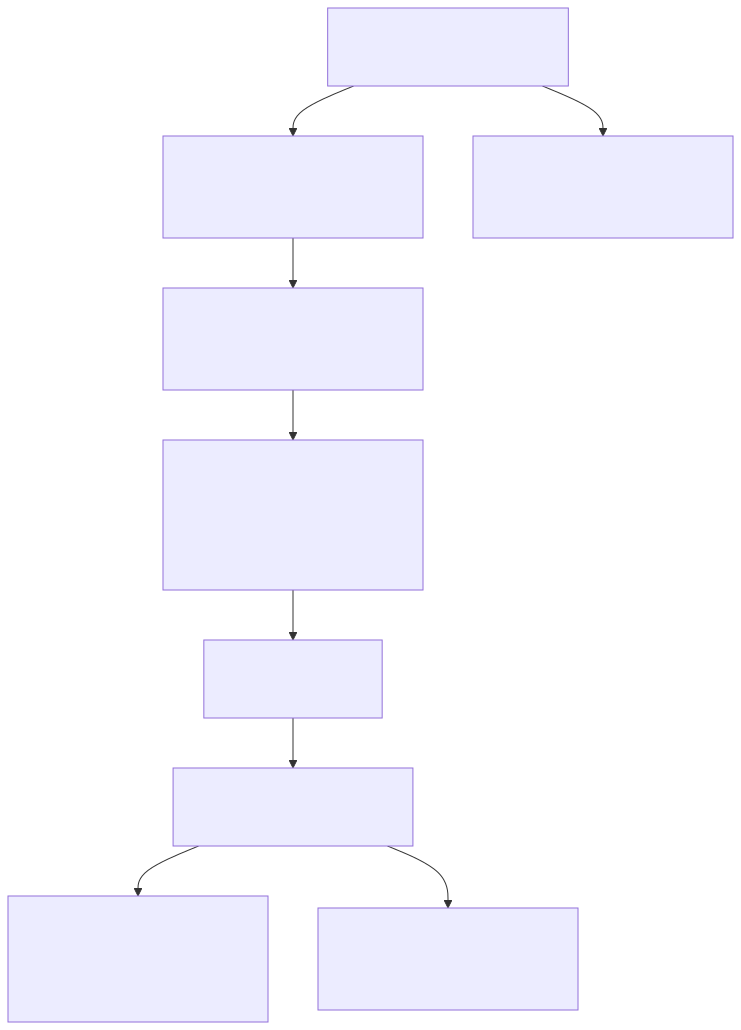
\includegraphics[keepaspectratio,width=\maxwidth,alt={Mermaid Diagram 1}]{generated/0009-session-start-protocol/mermaid_1.png}}

\begin{longtable}[]{@{}llll@{}}
\toprule\noalign{}
Field & Size & Description & Value \\
\midrule\noalign{}
\endhead
\bottomrule\noalign{}
\endlastfoot
\textbf{Version} & 1 byte & Protocol version & MUST be \texttt{0x02} for
version 2 \\
\textbf{Type} & 1 byte & Message type discriminant & See Message Types
table below \\
\textbf{Length} & 2 bytes & Payload length in bytes & 0-65535 \\
\textbf{Payload} & Variable & Message-specific data & CBOR-encoded where
applicable \\
\end{longtable}

\paragraph{4.2.1 Message Types}\label{421-message-types}

\begin{longtable}[]{@{}lll@{}}
\toprule\noalign{}
Type Code & Name & Description \\
\midrule\noalign{}
\endhead
\bottomrule\noalign{}
\endlastfoot
\texttt{0x00} & StartSession & Initiates a new session \\
\texttt{0x01} & SessionEstablished & Confirms session establishment \\
\texttt{0x02} & SessionError & Reports session establishment failure \\
\texttt{0x03} & KeepAlive & Maintains session liveness \\
\end{longtable}

\paragraph{4.2.2 Byte Order}\label{422-byte-order}

All multi-byte integer fields and values in the Session Start Protocol
MUST be encoded and interpreted in network byte order (big-endian). This
applies to:

\textbf{Protocol Message Fields:}

\begin{itemize}
\tightlist
\item
  \textbf{Length} field (2 bytes) in the common message format
\item
  \textbf{Challenge} field (8 bytes) in StartSession,
  SessionEstablished, and SessionError messages
\item
  \textbf{Additional Data} field (4 bytes) in StartSession messages
\item
  \textbf{Additional Data} field (8 bytes) in KeepAlive messages
\item
  \textbf{Session ID suffix} (64-bit) in HOPR Session ID format
\item
  Any future numeric fields added to the protocol
\end{itemize}

This requirement ensures consistent interpretation across different
architectures and prevents interoperability issues between
implementations.

\subsubsection{4.3 StartSession Message}\label{43-startsession-message}

Initiates a new session with the remote peer.

\pandocbounded{\includegraphics[keepaspectratio,width=\maxwidth,alt={Mermaid Diagram 2}]{generated/0009-session-start-protocol/mermaid_2.png}}

\begin{longtable}[]{@{}llll@{}}
\toprule\noalign{}
Field & Size & Description & Notes \\
\midrule\noalign{}
\endhead
\bottomrule\noalign{}
\endlastfoot
\textbf{Challenge} & 8 bytes & Random challenge for correlating
responses & MUST use CSPRNG \\
\textbf{Capabilities} & 1 byte & Session capabilities bitmap & See
Capability Flags table \\
\textbf{Additional Data} & 4 bytes & Capability-dependent options & Set
to \texttt{0x00000000} to ignore \\
\textbf{Target} & Variable & CBOR-encoded session target & e.g.,
"127.0.0.1:1234" \\
\end{longtable}

\paragraph{4.3.1 Capability Flags}\label{431-capability-flags}

\begin{longtable}[]{@{}lll@{}}
\toprule\noalign{}
Bit & Flag Name & Description \\
\midrule\noalign{}
\endhead
\bottomrule\noalign{}
\endlastfoot
0 & Reserved & Reserved for future use \\
1 & Reserved & Reserved for future use \\
2 & Reserved & Reserved for future use \\
3 & Reserved & Reserved for future use \\
4 & Reserved & Reserved for future use \\
5 & Reserved & Reserved for future use \\
6 & Reserved & Reserved for future use \\
7 & Reserved & Reserved for future use \\
\end{longtable}

\subsubsection{4.4 SessionEstablished
Message}\label{44-sessionestablished-message}

Confirms successful session establishment.

\pandocbounded{\includegraphics[keepaspectratio,width=\maxwidth,alt={Mermaid Diagram 3}]{generated/0009-session-start-protocol/mermaid_3.png}}

\begin{longtable}[]{@{}llll@{}}
\toprule\noalign{}
Field & Size & Description & Notes \\
\midrule\noalign{}
\endhead
\bottomrule\noalign{}
\endlastfoot
\textbf{Original Challenge} & 8 bytes & Challenge from StartSession
message & MUST match original challenge \\
\textbf{Session ID} & Variable & CBOR-encoded session identifier &
Assigned by responder, MUST be unique \\
\end{longtable}

\subsubsection{4.5 SessionError Message}\label{45-sessionerror-message}

Reports session establishment failure.

\pandocbounded{\includegraphics[keepaspectratio,width=\maxwidth,alt={Mermaid Diagram 4}]{generated/0009-session-start-protocol/mermaid_4.png}}

\begin{longtable}[]{@{}llll@{}}
\toprule\noalign{}
Field & Size & Description & Notes \\
\midrule\noalign{}
\endhead
\bottomrule\noalign{}
\endlastfoot
\textbf{Challenge} & 8 bytes & Challenge from StartSession message &
MUST match original challenge \\
\textbf{Reason} & 1 byte & Error reason code & See Error Codes table
below \\
\end{longtable}

\paragraph{4.5.1 Error Codes}\label{451-error-codes}

\begin{longtable}[]{@{}llll@{}}
\toprule\noalign{}
Code & Name & Description & Recommended Action \\
\midrule\noalign{}
\endhead
\bottomrule\noalign{}
\endlastfoot
\texttt{0x00} & Unknown Error & Unspecified error condition & Retry with
different parameters or node \\
\texttt{0x01} & No Slots Available & Exit node has no available session
slots & Retry later or try different node \\
\texttt{0x02} & Busy & Exit node is temporarily busy & Retry after brief
delay \\
\end{longtable}

\subsubsection{4.6 KeepAlive Message}\label{46-keepalive-message}

Maintains session liveness.

\pandocbounded{\includegraphics[keepaspectratio,width=\maxwidth,alt={Mermaid Diagram 5}]{generated/0009-session-start-protocol/mermaid_5.png}}

\begin{longtable}[]{@{}llll@{}}
\toprule\noalign{}
Field & Size & Description & Notes \\
\midrule\noalign{}
\endhead
\bottomrule\noalign{}
\endlastfoot
\textbf{Flags} & 1 byte & Reserved for future use & MUST be
\texttt{0x00} \\
\textbf{Additional Data} & 8 bytes & Flag-dependent options & Set to
\texttt{0x0000000000000000} to ignore \\
\textbf{Session ID} & Variable & CBOR-encoded session identifier & MUST
match established session \\
\end{longtable}

\subsubsection{4.7 Protocol Flow}\label{47-protocol-flow}

\pandocbounded{\includegraphics[keepaspectratio,width=\maxwidth,alt={Mermaid Diagram 6}]{generated/0009-session-start-protocol/mermaid_6.png}}

\subsubsection{4.8 Protocol Constants}\label{48-protocol-constants}

\begin{longtable}[]{@{}lll@{}}
\toprule\noalign{}
Constant & Value & Description \\
\midrule\noalign{}
\endhead
\bottomrule\noalign{}
\endlastfoot
\textbf{Protocol Version} & \texttt{0x02} & Current protocol version \\
\textbf{Default Timeout} & 30 seconds & Default session establishment
timeout \\
\textbf{Challenge Size} & 8 bytes & Fixed size for challenge field \\
\textbf{Max Payload Length} & 65535 bytes & Maximum message payload
size \\
\end{longtable}

\subsubsection{4.9 Protocol Rules}\label{49-protocol-rules}

\begin{longtable}[]{@{}lll@{}}
\toprule\noalign{}
Rule & Requirement Level & Description \\
\midrule\noalign{}
\endhead
\bottomrule\noalign{}
\endlastfoot
\textbf{Challenge Generation} & MUST & Challenge values MUST be randomly
generated using CSPRNG \\
\textbf{Session ID Uniqueness} & MUST & Session IDs MUST be unique per
responder \\
\textbf{Byte Order} & MUST & All multi-byte integer fields MUST use
network byte order \\
\textbf{CBOR Encoding} & MUST & Targets and Session IDs use CBOR
encoding {[}01{]} \\
\textbf{Payload Limits} & MUST & Messages MUST fit within HOPR packet
payload limits \\
\textbf{Keep-Alive Frequency} & SHOULD & KeepAlive messages SHOULD be
sent periodically \\
\textbf{Error Handling} & MUST & Implementations MUST handle all defined
error conditions gracefully \\
\textbf{Timeout Configuration} & SHOULD & Session establishment timeouts
SHOULD be configurable (default: 30s) \\
\end{longtable}

\subsubsection{4.10 Example Message
Exchanges}\label{410-example-message-exchanges}

\paragraph{4.10.1 Successful Session
Establishment}\label{4101-successful-session-establishment}

Complete session establishment with immediate keep-alive:

\pandocbounded{\includegraphics[keepaspectratio,width=\maxwidth,alt={Mermaid Diagram 7}]{generated/0009-session-start-protocol/mermaid_7.png}}

\paragraph{4.10.2 Session Establishment with
Error}\label{4102-session-establishment-with-error}

Session establishment failing due to resource exhaustion:

\pandocbounded{\includegraphics[keepaspectratio,width=\maxwidth,alt={Mermaid Diagram 8}]{generated/0009-session-start-protocol/mermaid_8.png}}

\paragraph{4.10.3 Session Establishment
Timeout}\label{4103-session-establishment-timeout}

Session establishment with no response from Exit Node:

\pandocbounded{\includegraphics[keepaspectratio,width=\maxwidth,alt={Mermaid Diagram 9}]{generated/0009-session-start-protocol/mermaid_9.png}}

\paragraph{4.10.4 Long-Running Session with Periodic
Keep-Alives}\label{4104-long-running-session-with-periodic-keep-alives}

Maintaining an established session over time:

\pandocbounded{\includegraphics[keepaspectratio,width=\maxwidth,alt={Mermaid Diagram 10}]{generated/0009-session-start-protocol/mermaid_10.png}}

\subsection{5. Design Considerations}\label{5-design-considerations}

\subsubsection{5.1 CBOR Encoding}\label{51-cbor-encoding}

The use of CBOR (Concise Binary Object Representation) for Session IDs
and Targets provides:

\begin{itemize}
\tightlist
\item
  Flexible data types without fixed-size constraints
\item
  Compact binary encoding
\item
  Language-agnostic serialization
\item
  Support for complex session identifiers
\end{itemize}

\subsubsection{5.2 Challenge-Response
Design}\label{52-challenge-response-design}

The 64-bit challenge provides:

\begin{itemize}
\tightlist
\item
  Correlation between requests and responses
\item
  Protection against replay attacks (when combined with transport
  security)
\item
  Simple state tracking for pending sessions
\end{itemize}

\subsubsection{5.3 Capability
Negotiation}\label{53-capability-negotiation}

The single-byte capability field allows:

\begin{itemize}
\tightlist
\item
  Up to 8 independent capability flags
\item
  Future protocol extensions
\item
  Backward compatibility through ignored bits
\end{itemize}

\subsubsection{5.4 Transport
Independence}\label{54-transport-independence}

The Session Start protocol is transport-agnostic:

\begin{itemize}
\tightlist
\item
  Works over any packet-based transport
\item
  Designed for HOPR packets but not limited to them
\item
  No assumptions about ordering or reliability
\end{itemize}

\subsubsection{5.5 Error Handling}\label{55-error-handling}

The protocol provides structured error reporting:

\begin{itemize}
\tightlist
\item
  Specific error codes for common failure scenarios
\item
  Challenge correlation for error attribution
\item
  Graceful handling of resource exhaustion
\end{itemize}

\subsection{6. Compatibility}\label{6-compatibility}

\subsubsection{6.1 Version
Compatibility}\label{61-version-compatibility}

\begin{itemize}
\tightlist
\item
  Version 2 is the initial protocol version
\item
  Future versions MUST use different version numbers
\item
  Implementations MUST reject messages with unknown versions
\item
  Version negotiation is out of scope for this specification
\end{itemize}

\subsubsection{6.2 Transport
Requirements}\label{62-transport-requirements}

\begin{itemize}
\tightlist
\item
  Requires bidirectional communication channel
\item
  No assumptions about ordering or reliability
\item
  Compatible with any transport providing packet delivery
\item
  Designed for HOPR mixnet but not limited to it
\end{itemize}

\subsubsection{6.3 Integration with HOPR Session Data
Protocol}\label{63-integration-with-hopr-session-data-protocol}

\begin{itemize}
\tightlist
\item
  HOPR Session Start Protocol establishes sessions for use by HOPR
  Session Data Protocol (see
  \href{../RFC-0008-session-protocol/0008-session-protocol.md}{RFC-0008})
\item
  Session IDs from this protocol are used to identify data sessions
\item
  Protocol operates independently but provides foundation for data
  exchange
\end{itemize}

\subsection{7. Security Considerations}\label{7-security-considerations}

\subsubsection{7.1 Protocol Security}\label{71-protocol-security}

\begin{itemize}
\tightlist
\item
  The protocol provides NO encryption or authentication
\item
  Security MUST be provided by the underlying transport
\item
  Session IDs SHOULD be unpredictable to prevent session hijacking
\item
  Challenges MUST use cryptographically secure random number generation
\end{itemize}

\subsubsection{7.2 Attack Vectors}\label{72-attack-vectors}

\begin{itemize}
\tightlist
\item
  Replay attacks possible without additional timestamp or nonce
  mechanisms
\item
  Man-in-the-middle attacks not prevented by protocol alone
\item
  Session targets may expose service information if not encrypted at
  transport
\item
  Resource exhaustion through excessive session establishment requests
\end{itemize}

\subsubsection{7.3 Mitigation
Strategies}\label{73-mitigation-strategies}

\begin{itemize}
\tightlist
\item
  Use transport-level security (e.g., HOPR packet encryption)
\item
  Implement rate limiting for session establishment requests
\item
  Use unpredictable session identifiers
\item
  Consider implementing session timeout mechanisms
\end{itemize}

\subsection{8. Future Work}\label{8-future-work}

\begin{itemize}
\tightlist
\item
  Session parameter renegotiation mechanisms
\item
  Performance optimizations for high-frequency session establishment
\end{itemize}

\subsection{9. Implementation Notes}\label{9-implementation-notes}

\subsubsection{9.1 Testing
Recommendations}\label{91-testing-recommendations}

\begin{itemize}
\tightlist
\item
  Test with various session target formats
\item
  Simulate network failures and timeouts
\item
  Verify challenge uniqueness and correlation
\item
  Test capability negotiation edge cases
\item
  Validate CBOR encoding/decoding correctness
\end{itemize}

\subsection{10. References}\label{10-references}

{[}01{]} Bormann, C. \& Hoffman, P. (2013).
\href{https://datatracker.ietf.org/doc/html/rfc7049}{Concise Binary
Object Representation (CBOR)}. \emph{IETF RFC 7049}.

\subsection{11. Related Links}\label{11-related-links}

\begin{itemize}
\tightlist
\item
  \href{../RFC-0011-application-protocol/0011-application-protocol.md}{RFC-0011
  Application Layer protocol}
\end{itemize}

\subsection{12. Appendix 1}\label{12-appendix-1}

Within HOPR protocol a Session is identified uniquely via HOPR Session
ID, this consists of a 10-byte pseudorandom bytes as prefix and 64-bit
unsigned integer as suffix. The 64-bit suffix is encoded and interpreted
as a big-endian unsigned integer.

In human readable format, a HOPR Session ID has the following syntax:

\texttt{0xabcdefabcdefabcdefab:123456}

The prefix represents a fixed pseudonym prefix of in the HOPR Packet
protocol (as in
\href{../RFC-0004-hopr-packet-protocol/0004-hopr-packet-protocol.md}{RFC-0004}).
The suffix represents an application tag that identifies Sessions within
the reserved range in the Application protocol
\href{../RFC-0011-application-protocol/0011-application-protocol.md}{RFC-0011}.
